\begin{figure}
\centering
\begin{tabular}{ccc}
%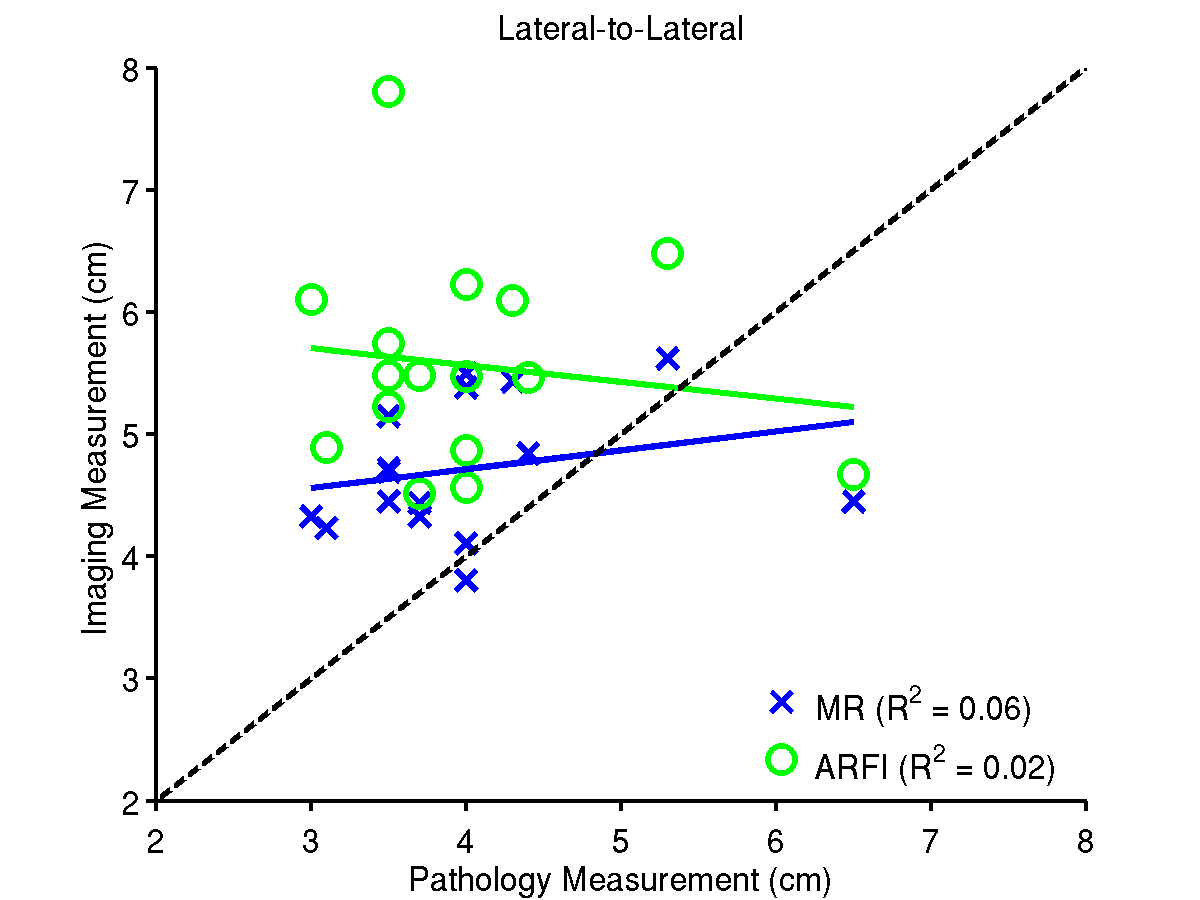
\includegraphics[width=0.3\linewidth]{figs/Lateral-to-Lateral} &
%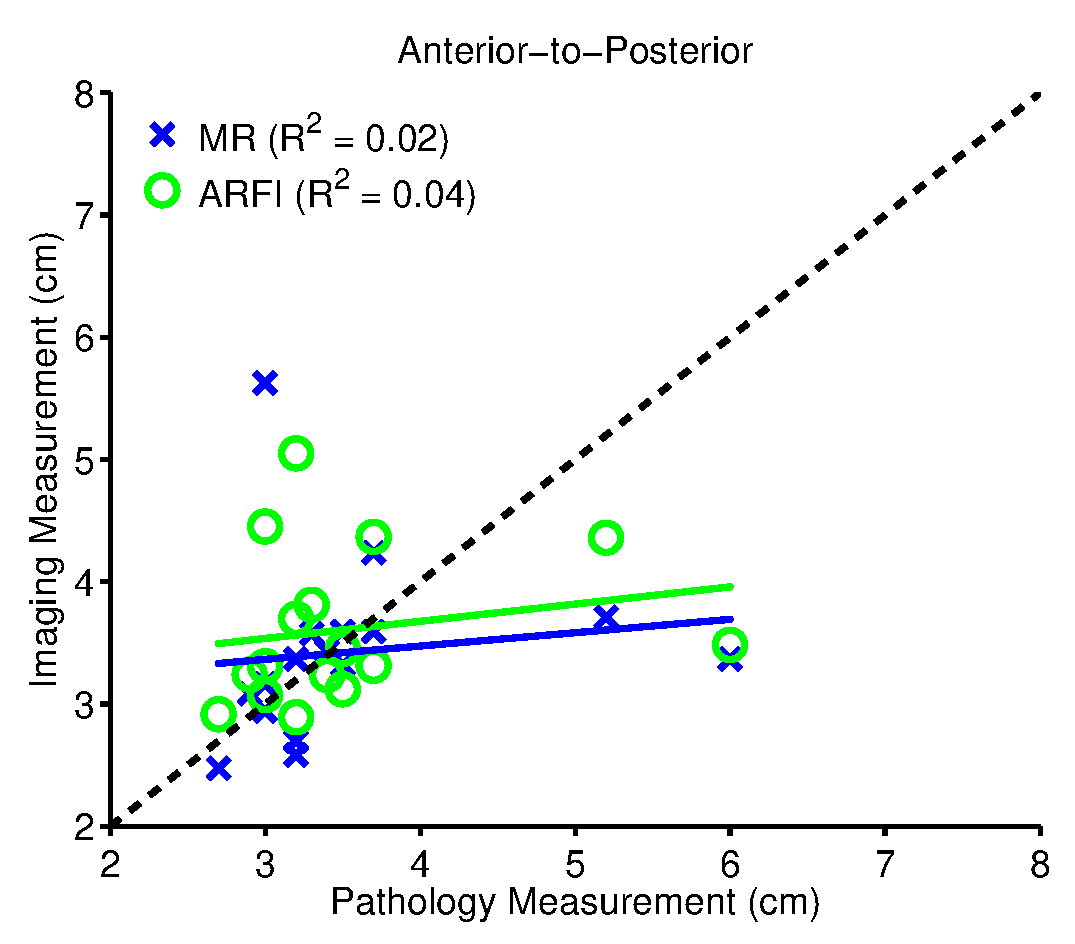
\includegraphics[width=0.3\linewidth]{figs/Anterior-to-Posterior} &
%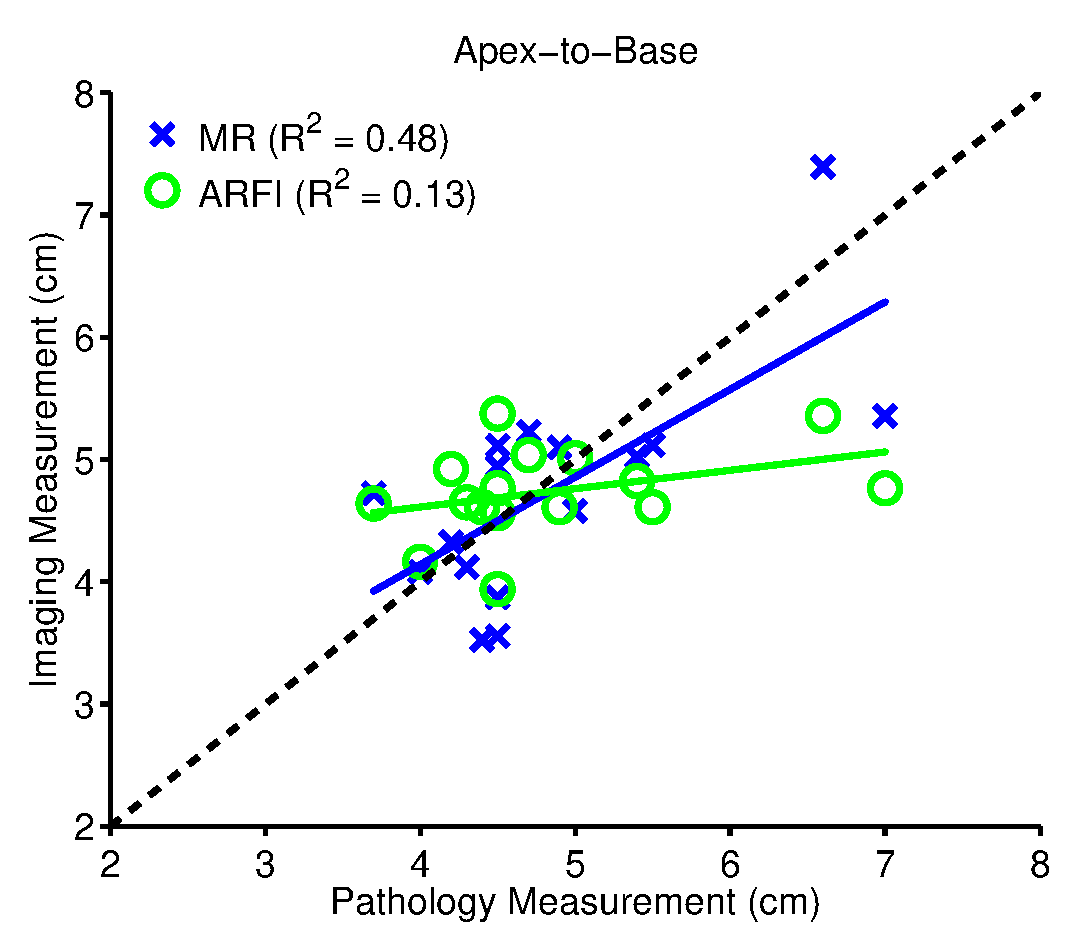
\includegraphics[width=0.3\linewidth]{figs/Apex-to-Base} \\
%(a) & (b) & (c) \\
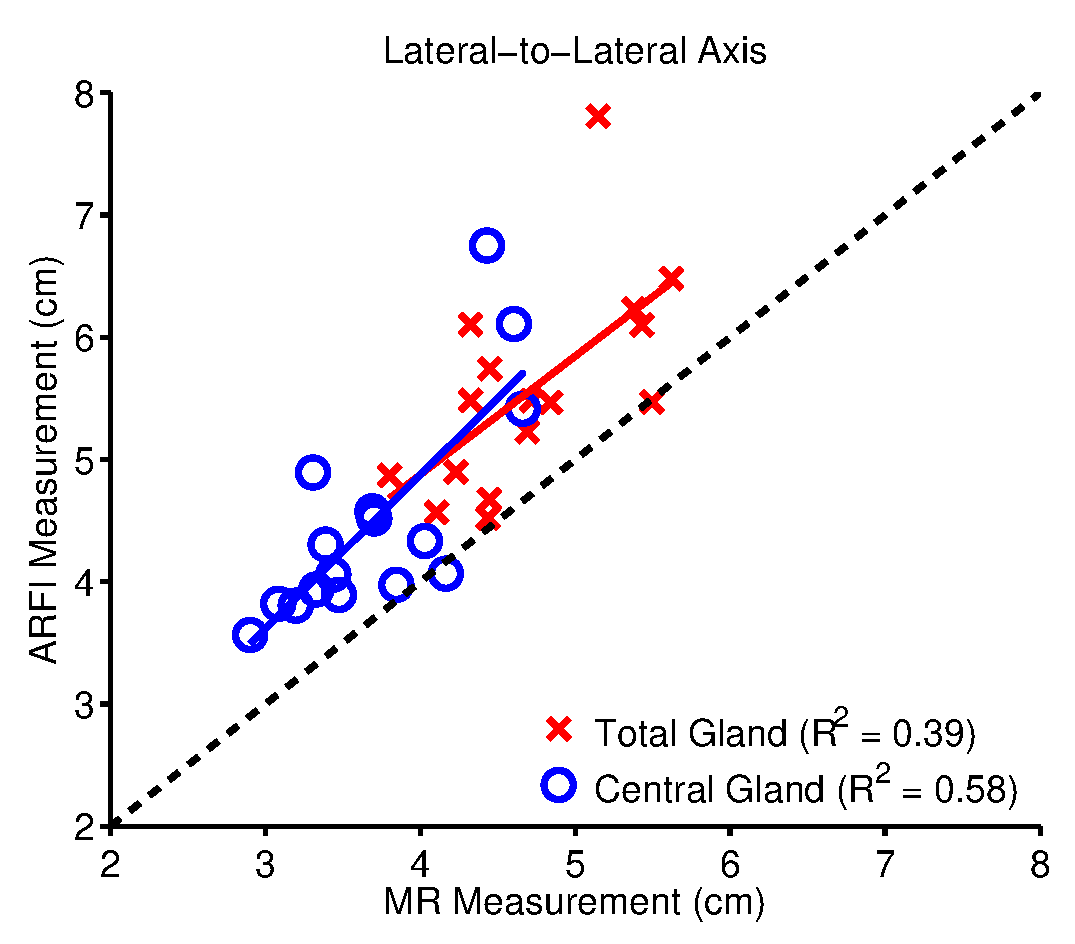
\includegraphics[width=0.3\linewidth]{figs/Imaging_Lateral-to-Lateral} &
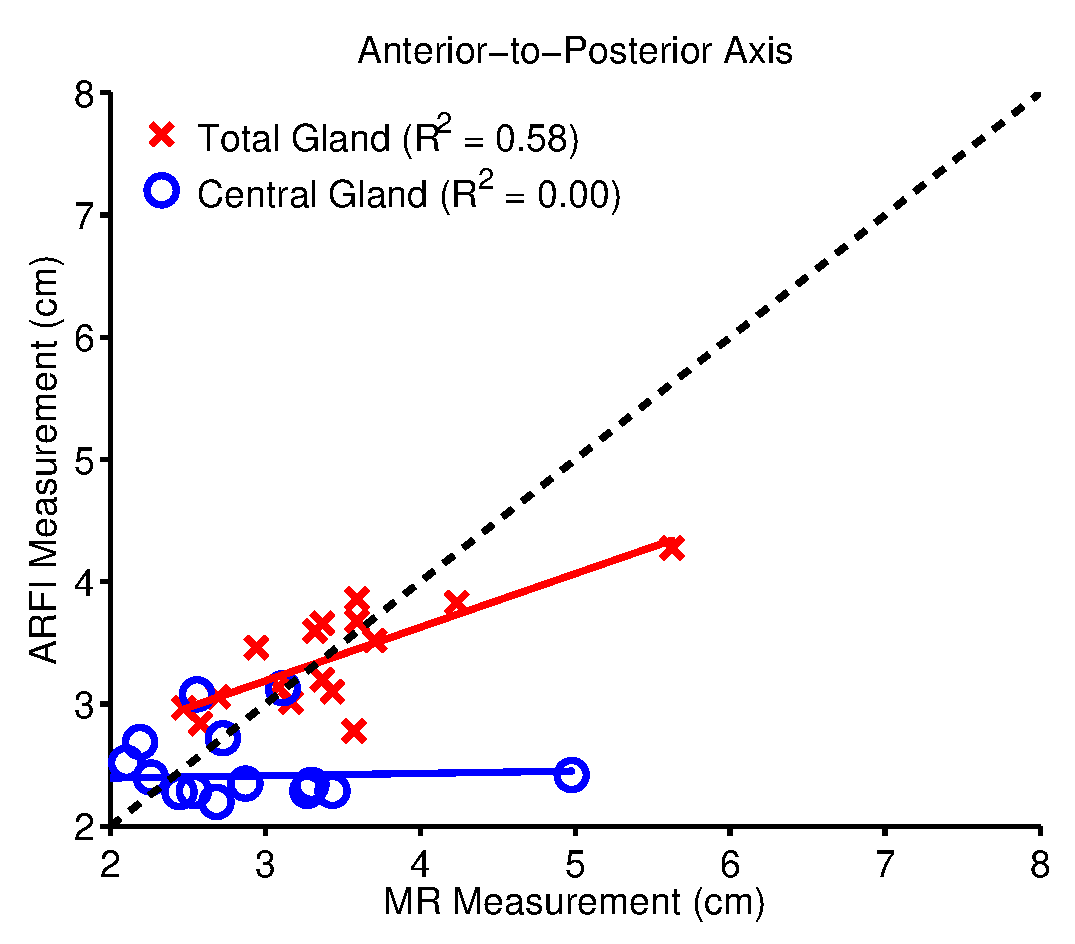
\includegraphics[width=0.3\linewidth]{figs/Imaging_Anterior-to-Posterior} &
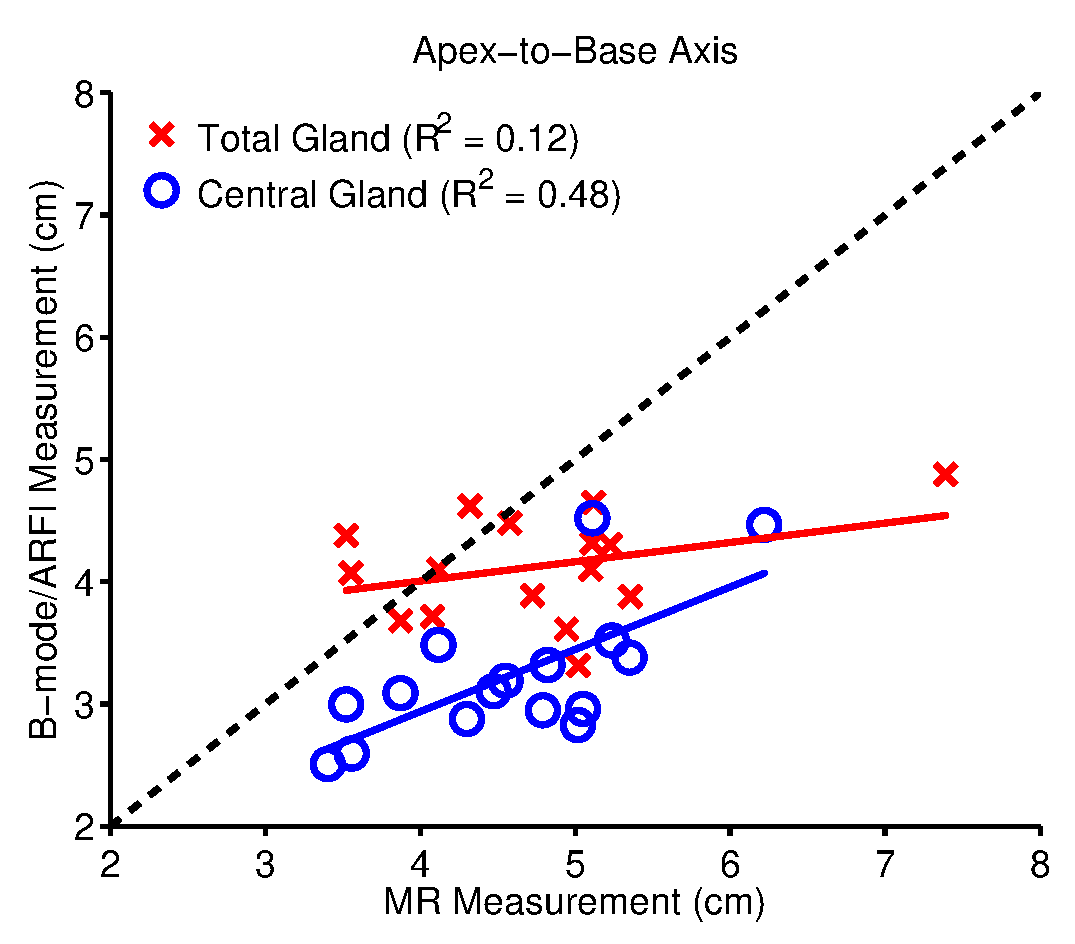
\includegraphics[width=0.3\linewidth]{figs/Imaging_Apex-to-Base} \\
(a) & (b) & (c) \\
%(d) & (e) & (f) \\
\end{tabular}
\caption{Measurements of the prostate dimensions along the three standard
    anatomic axes: lateral-to-lateral (a), anterior-to-posterior (b) and
    apex-to-base (c).  The correlation between the MR and B-mode/ARFI imaging
    axis measurements was performed in each orientation for the total gland
    (red crosses) and central gland (blue circles).  \textbf{B-mode images were
        used to estimate the total gland volume, and ARFI images were used to
        estimate the central glands.} The black dashed-line represents the
    projection of perfectly-correlated measurements between imaging and
    pathology.  The over-/under-estimation of each imaging modality relative to
    gross pathology and each other is summarized in
    Table~\ref{tab:mr_arfi_axes_error}.} 
\label{fig:mr_arfi_path_axes}
\end{figure}
